\chapter{基于攻击树的威胁建模}

\section{攻击树的构建}
在[协议]下的[攻击树]选项卡中有若干的攻击树面板,在窗体菜单[模型]或快捷按钮中均可添加新攻击树。
\par
点击小工具栏上的[创建攻击结点]、[创建与关系]、[创建或关系]、[创建非关系]和[创建顺序与关系]按钮,即可创建相应结点。
\par
其中,攻击结点带有对攻击的描述,绿色表示是一个安全结点(false),而红色表示该结点是可受攻击的(true)。顺序与关系和于关系具有相同的行为,只是语义不同,顺序与表示子结点的攻击应该按顺序依次发生,仅留作用户建模用。创建结点后如图\ref{attacktree_nodes}所示。
\begin{figure}[h]
	\centering
	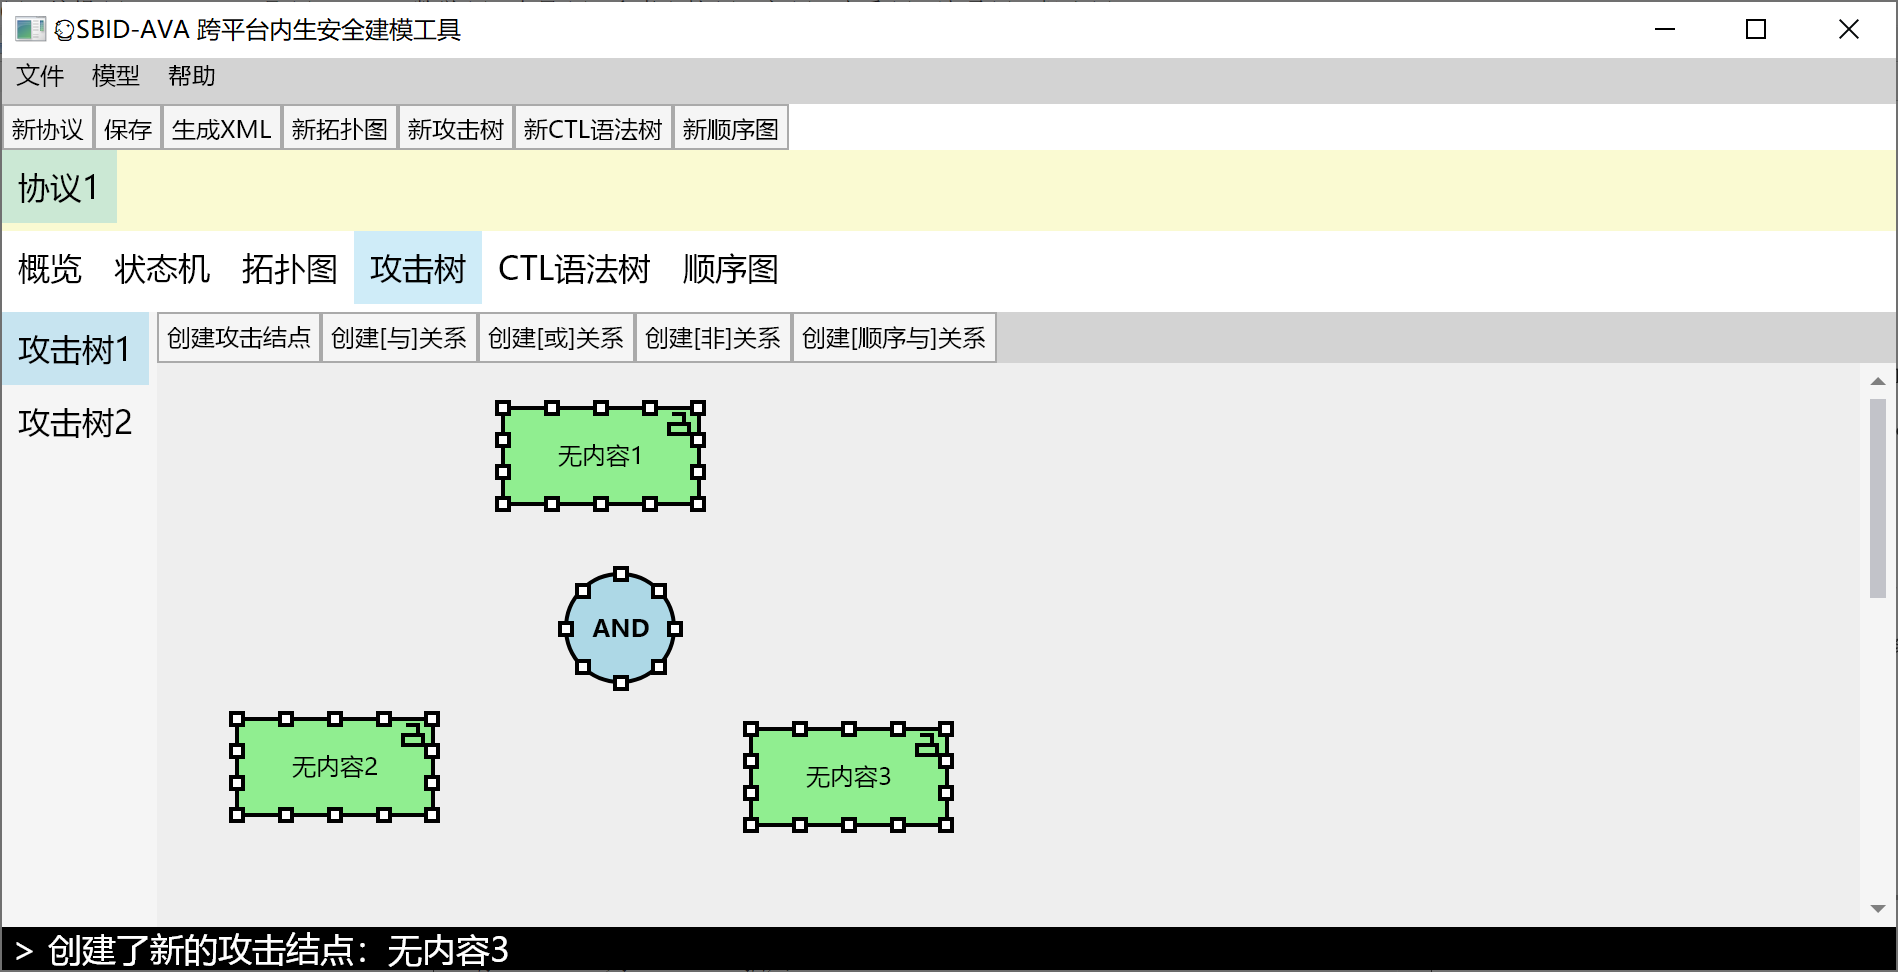
\includegraphics[width=12cm,height=6.75cm]{imgs/attacktree_nodes.png}
	\caption{创建结点}
	\label{attacktree_nodes}
\end{figure}
\par
在攻击结点上右键[编辑]即可编辑结点描述,[反转结点取值]可在受攻击和安全之间进行切换。攻击树的连线方式和状态机相同,先选择出发锚点,再点击要连线到的锚点即可。如图\ref{attacktree_simple}展示的是构建好的一棵简易攻击树。
\begin{figure}[h]
	\centering
	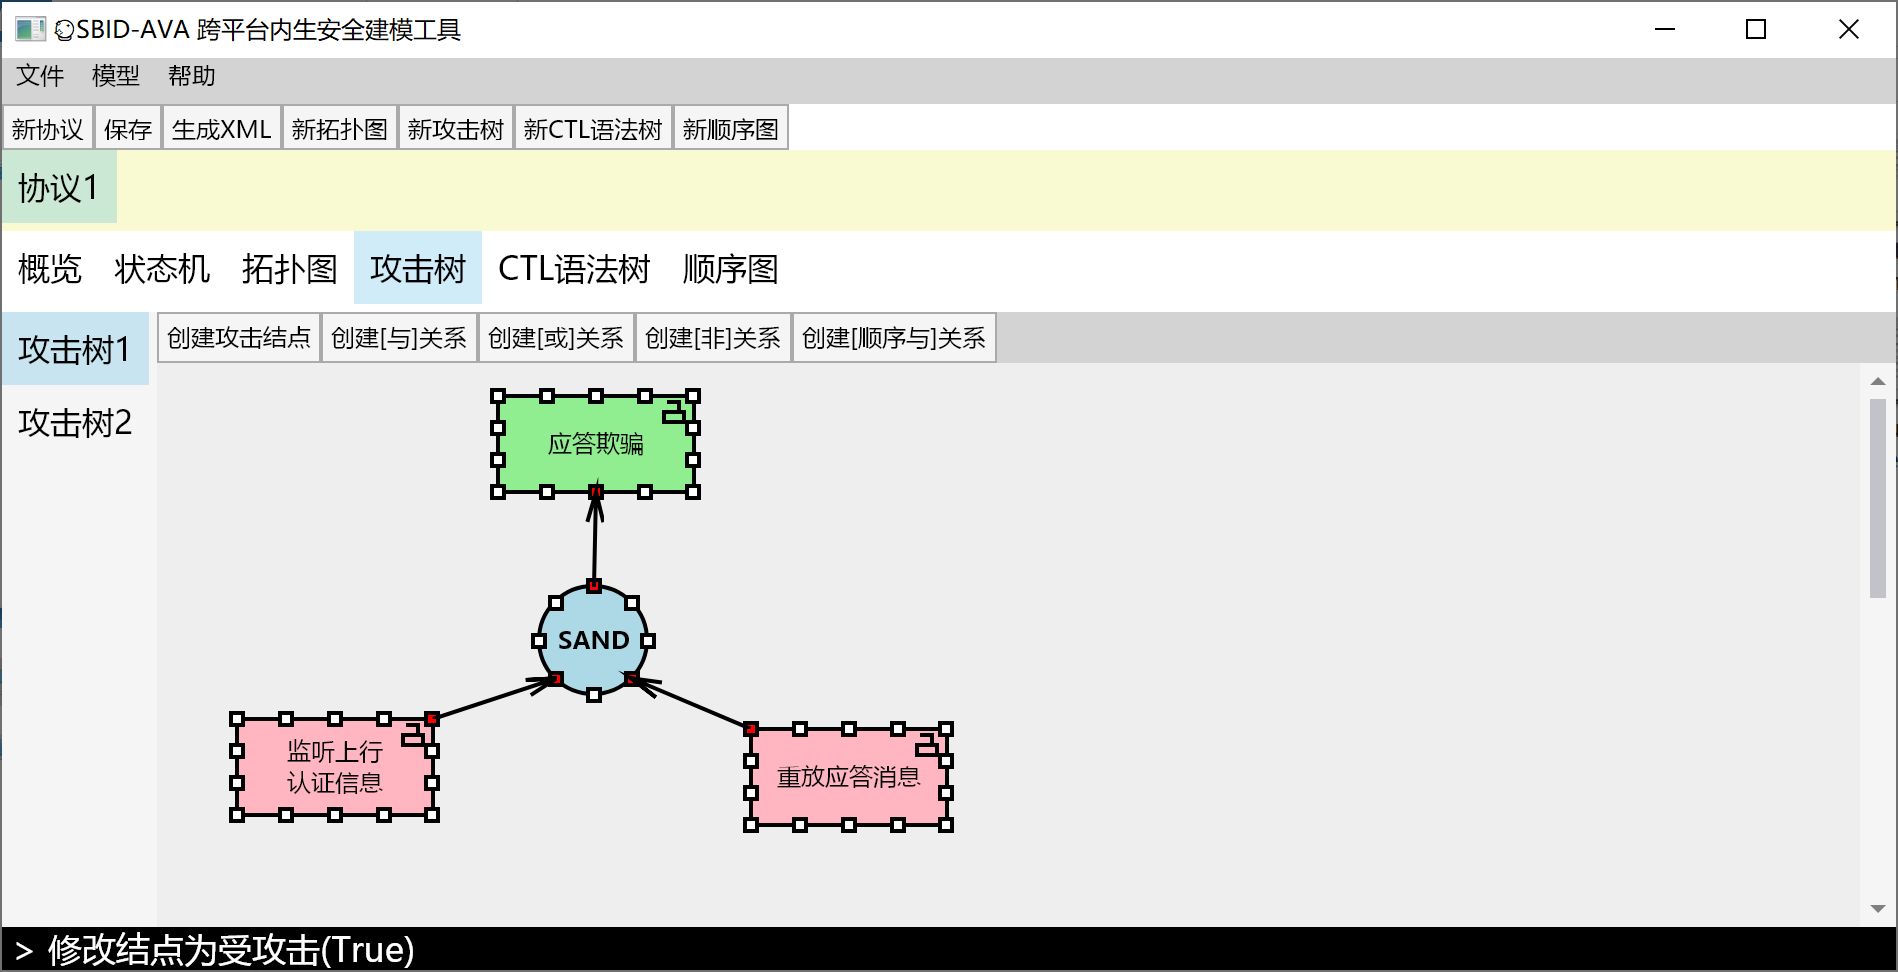
\includegraphics[width=12cm,height=6.75cm]{imgs/attacktree_simple.png}
	\caption{构建好的简易攻击树}
	\label{attacktree_simple}
\end{figure}

\section{威胁判定}
攻击树提供了一种正式而条理清晰的方法来描述系统所面临的安全威胁和系统可能受到的多种攻击。攻击树采用攻击-关系交替的多叉树结构来表达的攻击的产生逻辑,其中根节点表示攻击的目标,其它结点和结构表达了达成攻击目标的逻辑。
\par
攻击节点有两种状态:锁定的和活动的。
对于锁定的攻击结点,其值不会由子结点计算而来,总是取用当前值。
对于活动的攻击节点,其值由子节点计算得出。
可以通过点击攻击结点上的锁头标志切换锁定状态和活动状态。
\par
关系结点有四种,OR/AND/SAND/NEG,它们的计算逻辑如下。
\par
NEG结点:仅有一个子节点,子节点为TRUE则该结点为FALSE,子结点为FALSE则该结点为TRUE。
\par
AND和SAND结点:若子节点中有至少一个结点为FALSE,则该结点为FALSE,否则为TRUE。
\par
OR结点:若子节点中至少有一个结点为TRUE,则该结点为TRUE,否则为FALSE。
\par
攻击树构建完成后,右键点击要计算的的结点,选择[计算],则会通过子树计算出该结点的取值。如图\ref{attacktree_calculate}所示的例子中,由于两个子结点都是可攻击的,且它们之间的关系为顺序与,所以计算后的根结点也是可攻击的。
\begin{figure}[h]
	\centering
	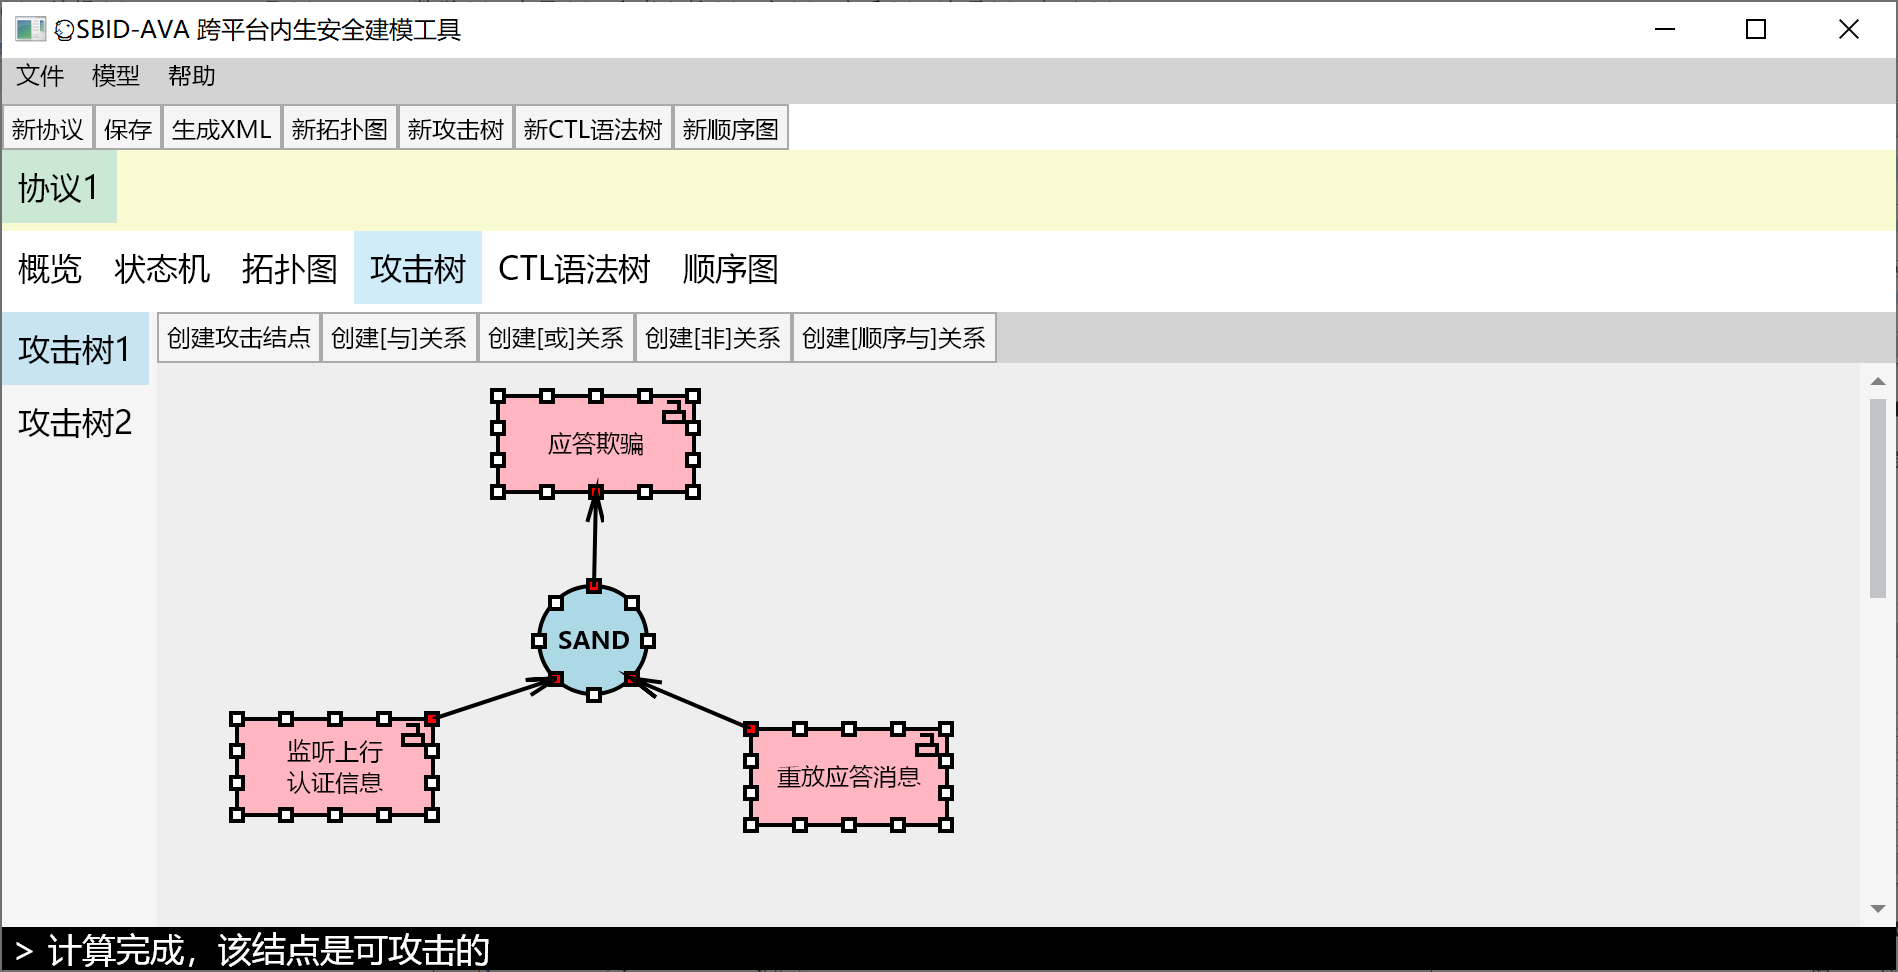
\includegraphics[width=12cm,height=6.75cm]{imgs/attacktree_calculate.png}
	\caption{威胁判定}
	\label{attacktree_calculate}
\end{figure}